\documentclass[12pt]{article}
\usepackage{notes-common}
\geometry{margin=0.35in}
\AtBeginDocument{\fontsize{14}{17}\selectfont}

% Mon Sep 28 -- Electric potential (V). Same lesson for both tracks (no
% calculus needed), so no PHYS 230/235 split. See
% electric-potential-notes-key.tex for the filled-in version -- same
% structure, wording and diagrams, every blank carries the answer.
%
% Built from Seth's rough notes (uploaded) + Knight Examples 25.6 and
% 25.9. Print layout matches electric-pe-notes.tex: small margins, bigger
% base font, blanks via \eqline (labeled line + its own rule below, for
% answers with real vertical extent) or \bl (short inline blank).
\newcommand{\eqline}[2][-0.5mm]{%
  \par\vspace{1mm}\noindent #2\par\vspace{#1}%
  \noindent\textcolor{rulehue}{\rule{\linewidth}{0.5pt}}\par\vspace{4mm}%
}

\begin{document}

\noteshead{Electric Potential}{}

\goal{
\begin{itemize}[itemsep=5pt,parsep=2pt,topsep=2pt]
\item See electric potential as charge's version of \emph{height}: PE per
charge, not PE itself.
\item Ask whether $V$ stays constant across a region where $\vec E$ is
constant (a parallel-plate capacitor) --- and check that against the same
question for gravity.
\item Convert between a potential difference and a change in speed
(Example 25.6).
\item Build $V$ for one point charge, then for several by \emph{adding
numbers}, not vectors (Example 25.9).
\end{itemize}}

%============================================================
\nsec{Electric potential is charge's ``height''}

A ball's gravitational PE isn't just a property of the ball --- you need two
more things:

\begin{itemize}[itemsep=6pt,parsep=3pt,topsep=3pt]
\item \bl[7cm]
\item Height \emph{relative to where}? \bl[5cm]
\end{itemize}

Electric potential energy works the same way. You need:

\begin{itemize}[itemsep=6pt,parsep=3pt,topsep=3pt]
\item \bl[7cm]
\item Potential \emph{relative to where}? \bl[5cm]
\end{itemize}

\textbf{Electric potential} is potential energy \emph{per charge} --- the
part of that pair that doesn't depend on which charge you put there:

\eqline{$V \equiv $}

measured in \bl[3cm], where $1\text{ V} = $ \bl[2.5cm].

\checkpoint{You're told $V=50$ V at some point. Can you find the PE a charge
would have there? What's missing?}

%============================================================
\nsec{Does $V$ stay constant where $\vec E$ is constant?}

A parallel-plate capacitor: two sheets of charge, surface density
$\pm\eta$, close together. Draw the field between and outside the plates.

\vspace{5.5cm}

\begin{itemize}[itemsep=6pt,parsep=3pt,topsep=3pt]
\item Each plate alone gives a field of magnitude \bl[3.5cm]
on either side of it.
\item Between the plates, the two fields point the \bl[2cm] direction and
add: $E_{\text{total}}=$ \bl[3cm] --- uniform, pointing from $+$ to $-$.
Outside the plates they \bl[2cm]: $E=0$.
\end{itemize}

\checkpoint{$\vec E$ is exactly constant everywhere between the plates.
Does that mean $V$ is constant there too? Compare to gravity: is
gravitational PE constant wherever the \emph{force} of gravity is constant?}

Sketch $V$ as you walk from the $+$ plate to the $-$ plate:

\begin{center}
\begin{tikzpicture}[x=1cm,y=1cm]
  \draw[gray!70, ->] (0,-0.4) -- (0,3.3) node[above, scale=0.8] {$V$};
  \draw[gray!70, ->] (-0.3,0) -- (7.3,0) node[right, scale=0.8] {position};
  \node[red!70!black, scale=0.8] at (0.4,-0.35) {$+$ plate};
  \node[blue!55!black, scale=0.8] at (6.6,-0.35) {$-$ plate};
\end{tikzpicture}
\end{center}

\begin{itemize}[itemsep=6pt,parsep=3pt,topsep=3pt]
\item The \bl[1.3cm] plate is at the higher potential.
\item $\vec E$ points from the $+$ plate to the $-$ plate --- i.e.\ toward
\bl[3cm] $V$. (Same rule as always: $\vec E$ points ``downhill.'')
\end{itemize}

%============================================================
\nsec{Worked example: crossing a potential difference}

\textit{A proton with speed $2.0\times10^5$ m/s enters a region where it
crosses a potential difference of $100$ V. What's its final speed? What if
it were an electron instead?}

Energy conservation, with $U=qV$:

\[
\tfrac12 m v_f^2 = \tfrac12 m v_i^2 - q\,\Delta V
\qquad\Longrightarrow\qquad
v_f =\
\]
\vspace{1.1cm}

\textbf{Proton} ($q=+e$, $m=1.67\times10^{-27}$ kg):

\eqline[0.2cm]{$(v_f)_p = $}

\textbf{Electron} ($q=-e$, much smaller $m$):

\eqline{$(v_f)_e = $}

\checkpoint{The proton slowed down; the electron sped up. Both crossed the
\emph{same} potential difference. Why the opposite result?}

%============================================================
\nsec{Potential of a single point charge}

Start from the PE of two point charges, and divide out the second charge
--- the same move that turned $U$ into $V$ up in \S1.

\[
U_{12} = \dfrac{1}{4\pi\varepsilon_0}\dfrac{q_1 q_2}{r_{12}}
\qquad\Longrightarrow\qquad
V_1 = \dfrac{U_{12}}{q_2} =\
\]
\vspace{1.0cm}

Given the potential of a point charge, what do you still need to get an
actual PE out of it?

\begin{itemize}[itemsep=6pt,parsep=3pt,topsep=3pt]
\item \bl[9cm]
\item \bl[9cm] --- a point charge's own potential already comes with a
reference built in: $V\to0$ as $r\to\infty$.
\end{itemize}

\checkpoint{As $r\to\infty$, what does $V_1$ approach? Does the \emph{sign}
of $q_1$ matter to $V_1$?}

%============================================================
\nsec{Potential from several charges: just add the numbers}

\textit{Example 25.9. A $+2.0$ nC charge is 5.0 cm from point $P$; a
$-1.0$ nC charge is 4.0 cm from $P$. Find $V$ at $P$.}

\begin{center}
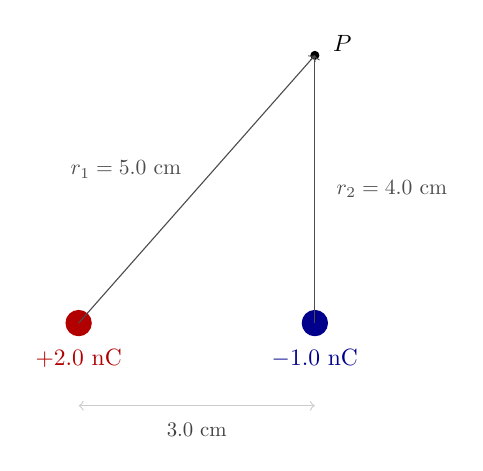
\begin{tikzpicture}[x=1cm,y=1cm]
  \coordinate (Pp) at (1.5,3.4);
  \filldraw[red!70!black] (-1.5,0) circle (0.16);
  \node[red!70!black, scale=0.85] at (-1.5,-0.45) {$+2.0$ nC};
  \filldraw[blue!55!black] (1.5,0) circle (0.16);
  \node[blue!55!black, scale=0.85] at (1.5,-0.45) {$-1.0$ nC};
  \filldraw[black] (Pp) circle (0.05);
  \node[scale=0.85] at (1.85,3.55) {$P$};
  \draw[gray!60!black, ->] (-1.5,0) -- (Pp);
  \node[gray!60!black, scale=0.78] at (-0.9,1.95) {$r_1=5.0$ cm};
  \draw[gray!60!black, ->] (1.5,0) -- (Pp);
  \node[gray!60!black, scale=0.78, anchor=west] at (1.68,1.7) {$r_2=4.0$ cm};
  \draw[gray!40, <->] (-1.5,-1.05) -- (1.5,-1.05);
  \node[gray!50!black, scale=0.75] at (0,-1.35) {$3.0$ cm};
\end{tikzpicture}
\end{center}

The potential is a \emph{scalar} --- no angles, no components. Just add the
two numbers:

\[
V = V_1 + V_2 = \dfrac{1}{4\pi\varepsilon_0}\dfrac{q_1}{r_1}
+ \dfrac{1}{4\pi\varepsilon_0}\dfrac{q_2}{r_2}
\]

\eqline[0.2cm]{$V_1 = $ \hspace{4.5cm} $V_2 = $}

\eqline{$V = $}

\checkpoint{Suppose you needed $\vec E$ at $P$ instead of $V$. Would this
same ``just add the numbers'' shortcut work?}

\end{document}
